\documentclass[a4paper,11pt]{article} % Artículo porque a la hora de poner los títulos los enumera con 1., 2.,... sin embargo el report te los enumera así: 0.1., 0.2.,...
\usepackage[T1]{fontenc}
\usepackage[utf8x]{inputenc} % Esto hace que latex interprete la codificación del documento como utf-8 sin dar errores en las tildes
\usepackage[spanish]{babel} % Para poner el idioma en castellano(fecha,Índice...)
\usepackage{graphicx} %Para las imagenes
\usepackage{caption} %Para los textos de las imágenes
\usepackage{subcaption} % Para los textos de las imagenes tengan varios apartados
%Estas dos líneas (esta y la de abajo)ponen interlineado 1,5 excepto en notas a pie de página e igual algo más (que no sé)
\usepackage{setspace} % Paquete para interlineado.
\onehalfspacing % Interlineado a 1'5
%\usepackage{helvet}
%\renewcommand{\familydefault}{\sfdefault}
%\usepackage{uarial}
%\renewcommand{\familydefault}{\sfdefault}
\usepackage[nottoc,numbib]{tocbibind}

\usepackage[top=2.5cm, left=4cm, bottom=2.5cm, right=3cm]{geometry} % Para los márgenes

\usepackage{color} % Para poder poner las letras en color si es necesario
\usepackage[toc,page]{appendix} % Para poder poner los Anexos
\renewcommand{\appendixname}{Anexos} %Para cambiar de nombre los appendices por anexos
\renewcommand{\appendixtocname}{Anexos} %Para cambiar de nombre los appendices por anexos
\renewcommand{\appendixpagename}{Anexos} %Para cambiar de nombre los appendices por anexos
\newcommand*{\Appendixautorefname}{}

\usepackage[colorlinks=true, linkcolor=blue, citecolor=red, linktoc=page]{hyperref} % Para poner links
\usepackage{float}

% Páginas abajo a la derecha
\usepackage{fancyhdr}
\fancyhf{} % clear all header and footers
\renewcommand{\headrulewidth}{0pt} % remove the header rule
\rfoot{\thepage}

%\usepackage[]{adjustbox}

% Solución para colisiones entre hyperref y appendix
\usepackage{etoolbox} 
\makeatletter
\appto{\appendices}{\def\Hy@chapapp{Appendix}}
\makeatother
% % % % % % % % % % % % % % % % % % % % % % %
\usepackage{ccicons}
\usepackage{titlepage}
\begin{document} % Siempre hay que ponerlo
\pagestyle{empty}
\title{Anatomía de superficie: su representación pictórica en la muerte de Cristo}
\author{Nerea González Cordero}
\date{\today}
\maketitle % Para crear la portada
\newpage % Para salto de página

\textbf{Resumen}

La muerte de Cristo, siendo una gran desconocida excepto por las distintas narraciones de los evangelios, es un tema muy recurrido en el arte. Analizando varias obras se aprecia un recorrido histórico de la representación anatómica y de la muerte de Cristo, siendo éstas variables según las distintas creencias, percepciones sociales y religiosas e ideales de belleza de cada momento histórico.

Mediante el estudio de cuatro obras pictóricas se observan las variaciones en la anatomía de superficie de las figuras representadas, según el conocimiento anatómico de la época que actúa como principal factor influyente. Pudiendo examinar desde las proporciones seguidas por el artista, hasta las características menos humanas y más divinas con las que algunos autores nos fascinan.

Además, se pueden distinguir las diferentes percepciones de Cristo en varias épocas en cuanto a la representación de su gloria, como hijo de Dios y Dios, o su muerte, más humana, respectivamente.

\vspace{15pt}

\textbf{Palabras Clave:}
Anatomía de superficie, Cristo, crucifixión, obra pictórica, muerte.

\vspace{30pt}

\textbf{Abstract}

The death of Christ, being a great unknown except for all the accounts in the Gospels, is one of the more recurrent topics in art. Analizing some artworks it is noticeable a historical path of the anatomical representation and of th e death of Christ, those of whom are changeable according to th different beliefs, social and religious perceptions and beauty ideals from each period of time.

By the study of four works of art, it is observable the variations on the surface anatomy of the represented figures, according to the anatomical knowledgement in each epoch, which acts as the main influential factor. It can be exhaminated from the proportions given by the artist until the less human features and the more divine ones some authors fascinate us with.

Furthermore, the different perceptions of Christ can be distinguished  along the time, refering to his glory representation, as son of God and God, or even his death, more human, respectively.

\vspace{15pt}

\textbf{Key words:}
Surface anatomy, Christ, crucifixion, artwork, death.
\tableofcontents % Para el Índice
\newpage

\pagestyle{fancy} % Empezar a numerar
\pagenumbering{arabic} % La numeración de las páginas, también se puede con números romanos {roman}

\section{Introducción} % Para los títulos
El arte podría definirse como una expresión de la creatividad humana que produce obras apreciadas por su belleza o emotividad y que es innata en el ser humano \footnote{Definición según el Diccionario Oxford: www.oxforddictionaries.com/definition/english/art}. Existe desde el origen del ser humano y  % (http://www.oxforddictionaries.com/definition/english/art)
a lo largo de los siglos ha ido evolucionando hasta el arte contemporáneo. Junto con las obras artísticas también se han ido transformando las representaciones anatómicas en las obras pictóricas y escultóricas.

La anatomía de superficie es la ciencia que estudia las características anatómicas que pueden ser estudiadas mediante la vista y la palpación \footnote{Definición según Wikiradiography: www.wikiradiography.com/page/Surface+Anatomy}% (http://www.wikiradiography.com/page/Surface+Anatomy)
, es decir, la superficie del cuerpo. En el caso de la anatomía humana estudia desde las proporciones del cuerpo hasta puntos de referencia visibles en el exterior que están relacionados con órganos y partes internas, tanto en pose estática como en movimiento. % (http://www.princeton.edu/~achaney/tmve/wiki100k/docs/Superficial\_anatomy.html)
% %http://www.theodora.com/anatomy/surface\_anatomy\_index.html

%Como la materia principal de mi trabajo es la antomía de superficie relataré lo más relevante acerca de cómo ha evolucionado el conocimiento de esta materia hasta llegar al conocimiento actual.
\subsection{Historia de la anatomía}
A lo largo de la historia ha habido diferentes impedimentos que han provocado que hasta épocas muy recientes la anatomía del cuerpo humano fuese una gran desconocida, incluso entre aquellos que fundamentalmente trabajaban vinculados al cuerpo humano por distintas razones, como pueden ser médicos o artistas.

Desde el antiguo Egipto se ha estudiado la anatomía del ser humano, aunque no estaba a la altura del desarrollo médico que poseían, posiblemente por el gran respeto que profesaban a los cadáveres. Conocían algunas estructuras como el corazón, el cual consideraban el órgano central y lugar del pensamiento y los sentimientos, el hígado, el bazo, los riñones e incluso la existencia de vasos sanguíneos que transportaban distintos fluidos.

Los griegos fueron los grandes anatómicos de la antigüedad, de hecho, se recogen bastantes textos médicos en el Corpus Hipocraticum \footnote{Colección de trabajos médicos elaborados en la antigua Grecia. A pesar de su nombre no está comprobado que Hipócrates sea el autor de todos estos escritos, de hecho se desconoce el autor de la mayoría de ellos.}. En estos se describen la función de algunos órganos, así como del sistema músculo-esquelético y también la diferencia entre arterias y venas. Fueron los primeros en formar escuelas de anatomía e incluso los primeros en diseccionar cuerpos humanos \footnote{Ptolomeo I fue el primero que aprueba la utilización de cuerpos humanos para su disección y estudio anatómico. Durante su reinado y el de su dinastía fue posible para algunos anatomistas la realización de disecciones. El más importante es Herófilo considerado como "Padre de la anatomía".}, lo que permitió un conocimiento más avanzado del cuerpo humano. Sin embargo, esto no era lo habitual y normalmente utilizaban sus conocimientos de las disecciones de animales para aplicarlos a la anatomía humana.

Galeno siguió con los estudios anatómicos mediante la disección de animales aportando además otros conocimientos que recibía gracias a su condición de médico entre los gladiadores donde podía vislumbrar cualquier tipo de herida. Sus estudios se encuentran recogidos en sus numerosos tratados. \footnote{Galeno con más de 500 tratados fue el autor de la antigüedad que más escritos elaboró.}

En otras culturas como la india y la china la anatomía tampoco estaba más desarrollada que la occidental, que se basó durante varios siglos en los tratados galénicos.

El conocimiento anatómico del ser humano apenas avanzó en occidente durante la Edad Media, debido a la creencia cristiana de que el alma de un cuerpo diseccionado no podría ir al ``Cielo". Por ello las disecciones fueron un tema tabú durante esta época, y desapareció el interés por el cuerpo concentrándose éste en el alma. La cultura islámica poseía un conocimiento médico muy desarrollado para la época, sin embargo las disecciones de cadáveres humanos estaban prohibidas, por lo que su conocimiento de anatomía se basaba en las disecciones de animales y no era muy superior al de la Europa cristiana.

%Posteriormente, ya en la Edad moderna, se conceden permisos para diseccionar cadáveres de criminales como una parte más de la pena por su delito.

No es hasta Leonardo Da Vinci que se empezaron a hacer verdaderos progresos en la anatomía humana. Sus conocimientos se debieron a disecciones que llevó a cabo en cuerpos humanos y están plasmadas en una gran variedad de dibujos \footnote{El Hombre de Vitruvio es la más conocida de todas las ilustraciones elaboradas por Da Vinci (ver anexo \autoref{app:vitruvio}).}. Aunque el verdadero cambio de la anatomía galénica a una doctrina más moderna se dio en el siglo XVI gracias a Andrés Vesalio. Éste es el autor de "De Humani Corporis Fabrica", donde se recogen diversos dibujos de anatomía humana (ver anexo \autoref{app:vesalio}). Vesalio, junto con otros personajes influyentes de la época y posteriores como Miguel de Servet o William Harvey, provocó una auténtica revolución en la anatomía tradicional.

%Además, a partir de este momento los estudiantes de anatomía no tenían que saber latín para poder estudiar y lo podían hacer mediante las diversas representaciones que se estaban llevando a cabo.

Las disecciones empezaron a ser más comunes, y se observaron varios problemas.

El primer problema se debía a la temperatura del ambiente. En aquella época no se conocía la manera de conservar un cuerpo. Es por esto que la disecciones se podían realizar exclusivamente en los meses de temperatura más baja, cuando el frío mantenía el cadáver por más tiempo. Aún así había que realizar la disección casi inmediatamente después de la muerte del individuo, pues los cuerpos no tardaban mucho en descomponerse.

El segundo problema provenía del aumento de las disecciones. Debido a los pocos cuerpos que  se permitían diseccionar y al aumento de estudiantes de anatomía se empezaron a profanar tumbas para conseguir cadáveres, algunos incluso llegaron más lejos matando a personas para vender sus cuerpos \footnote{Son conocidos los asesinatos de West Port o de Burke y Hare que fueron llevados a cabo durante 1828 en Edimburgo. William Burke y William Hare asesinaron a dieciséis personas y vendieron sus cuerpos al Doctor Robert Knox, quien los utilizaba en sus clases de anatomía. Cuando se descubrieron los crímenes Hare testificó contra Burke quien fue condenado a muerte y después diseccionado.}.

Para evitar este último problema se elaboró la ley de anatomía de 1832 (Reino Unido) que regulaba las donaciones de cuerpos a la ciencia y la obtención de licencias para obtener el permiso que permitía diseccionar cadáveres.

%Durante los siglos XVII y XVIII el campo de la anatomía se desarrolla tremendamente. Al principio se realizaban disecciones en plazas donde cualquiera podía atender a la explicación de un maestro, después, no obstante las disecciones pasan a realizarse en aulas siendo muchos menos los beneficiados que aprendían anatomía.

En los siglos XIX y XX el conocimiento anatómico adquirió su completa madurez gracias al avance de otras disciplinas científicas y tecnológicas que ayudaron a ello.
% http://www.bl.uk/learning/artimages/bodies/vesalius/renaissance.html
% http://www.sciencemuseum.org.uk/broughttolife/themes/understandingthebody/dead.aspx
% http://en.wikipedia.org/wiki/Anatomy\_Act\_1832
% http://en.wikipedia.org/wiki/Cadaver
% http://en.wikipedia.org/wiki/History\_of\_anatomy
% http://en.wikipedia.org/wiki/Hippocratic\_Corpus
% http://en.wikipedia.org/wiki/Galen
% Historia de la anatomía. Dr José Alfredo Sillau Gilone (en descargas 3 partes: libro de historia de la anatomía, historia anatomía e historia de la anatomía.)


\subsection{Muerte de Cristo}
La muerte de Cristo es una tema muy recurrido en la obra pictórica. En los siglos inmediatamente posteriores a la crucifixión no representaban tal cual al Cristo en la cruz, sino que lo hacían mediante otros símbolos y más tarde exclusivamente la cruz. Fue, sobre todo, a partir de la Edad Media (siglo V) cuando empezó a ser frecuente la imagen del Cristo crucificado.

Por otra parte, la iconografía cristiana varía de forma y estilo según las percepciones de la época artística en la que se desarrolla, en la que predomina un estilo determinado, pero en todas ellas ha tenido gran relevancia. De un joven imberbe se pasa a un hombre con barba. Ambas representaciones confluyen, pero artísticamente al final persiste la segunda. También se pasa de una visión de un Cristo triunfal a una visión más humana y menos divina de Cristo en el suplicio de la crucifixión.

Puesto que fue el emperador Constantino quien abolió la crucifixión en el siglo IV d.C, y no hay documentación ni representaciones acerca de ello hasta varios siglos después, es difícil saber cómo era, en la época romana, esta pena capital, que se utilizaba únicamente para los peores delincuentes.

Se sabe que aunque ha habido distintas formas de crucifixión, los romanos del periodo comprendido alrededor del nacimiento y la muerte de Cristo utilizaban la cruz \textit{commisa}, vulgarmente denominada cruz latina que es la más frecuentemente representada, o la cruz \textit{immissa}, en forma de T (ver anexo \autoref{app:crosses}). Éstas estaban formadas por dos tablones de madera: un poste vertical que se insertaba en el suelo, que recibe el nombre de \textit{stipes} y un travesaño horizontal denominado \textit{patibulum}. A veces en la mitad del poste vertical se insertaba un bloque de madera que servía de asiento. También se utilizaba, aunque probablemente posteriormente al tiempo en el que vivió Cristo, un tablón que colocado a la altura de los pies ejercía de apoyo para éstos.

Dependiendo de la altura de las cruces éstas se dividían en la \textit{cruz humilde}, la más habitualmente usada, cuya altura era de unos dos metros y la \textit{cruz sublime}, tan alta que los pies del condenado se encontraban aproximadamente a un metro del suelo. Se cree que Cristo pudo haber sido crucificado en una de estas últimas ya que necesitaron una caña para poder acercarle la esponja con vinagre cuando estaba al borde de la muerte (Mt 27, 48; Mc 15, 36; Jn 19, 29). En este aspecto, muchas de las representaciones que podemos observar de crucifixiones de Cristo podrían ser correctas.

Diversas fuentes dejan claro que los romanos utilizaban clavos para sujetar a los individuos crucificados a la cruz \footnote{Así como los evangelios atestiguan que Jesús fue clavado en la cruz, otros autores coetáneos se refieren también al uso de los clavos en la crucifixión. Ejemplos de ello son Séneca y Tranión. Además, las únicas reglas jurídicas que se conocen desde 1967 referentes a la crucifixión dan a entender que a los crucificados se les clavaba en la cruz.}. Además, la crucifixión variaba según la región y la inventiva del verdugo.

La creencia más extendida actualmente es la de que los clavos eran introducidos a la altura de la línea de flexión  de la muñeca, entre el cúbito y el radio y justo entre estos y los carpos o entre las dos filas de huesos metacarpianos. Se ha llegado a esta conclusión tras haber encontrado hallazgos arqueológicos de esa época que concuerdan con esta teoría y tras la realización de experimentos que apuntan a esta misma conclusión\footnote{El doctor Pierre Barbet realizó una serie de experimentos con cadáveres en los que se demostraba esta teoría.}. Anteriormente se creía que los clavaban en las manos porque así lo establece Juan en su Evangelio (Jn 20, 20-29), sin embargo ha de tenerse en cuenta que, antiguamente, la muñeca se encontraba en lo que se denominaba ``mano", que abarcaba hasta el brazo, lo que ha podido inducir a error durante siglos.

En cuanto a la técnica de clavado de los pies, no está claro si realizaban la inserción de los clavos juntando ambos pies y utilizado para ello un solo clavo, o la fijación de éstos se llevaba a cabo por separado mediante dos clavos. Probablemente los clavos eran insertados entre el segundo y tercer metatarsiano. En las representaciones pictóricas se emplea tanto la imagen de Cristo crucificado mediante tres clavos como mediante cuatro.

Teniendo en cuenta las dificultades en el conocimiento de la crucifixión de Cristo es lógico pensar que en la mayoría de la iconografía referente al tema Cristo es representado según el gusto y estilo de cada autor claramente ubicado en su época.

% Enciclopedia moderna, 11: diccionario universal de literatura, ciencias, artes, agricultura, industria y comercio. Francisco de Paula Mellado (Pág:805-811)
% http://www.frugalsites.net/jesus/crucifixion.htm
% http://mb-soft.com/believe/text/crucifix.htm
% LA CRUCIFIXIÓN Laura RODRÍGUEZ PEINADO (en documentos del TFG)
% http://www.shroud.com/bucklin2.htm

Si existe debate acerca de si Jesús murió verdaderamente en la cruz \footnote{Algunos autores como Margaret y Trevor Lloyd Davies, los mayores defensores, consideran la posibilidad de que Jesucristo no muriese verdaderamente en la cruz. Otro ejemplo de esta hipótesis se encuentra reflejada en el libro \textit{42 días, Análisis forense de la crucifixión y la resurrección de Jesucristo}, de Miguel Lorente.}, aún es mayor el debate existente sobre la presunta causa de su muerte.

Existen varias teorías al respecto:

1) Embolia Pulmonar

2) Rotura cardíaca

3) Trauma de suspensión

4) Asfixia

5) Herida perforante fatal

6) Shock

7) Síncope fatal

8) Arritmia cardíaca

9) Coagulopatía inducida por traumatismos.

Todas estas hipótesis han sido analizadas en profundidad, no llegando, sin embargo, a la conclusión acerca de cuál es la real. Lo que está claro, sin embargo, es que Cristo padeció terribles sufrimientos, los cuales en conjunto pudieron conducirle a su muerte, que se produjo hacia las tres de la tarde tras varias horas en la cruz.

% The Search for the Physical Cause of Jesus Christ's Death Author: W. Reid Litchfield Categories: God and Jesus Christ, Science Journal: 37:4 (en documentos de TFG)
% The crucifixion of Jesus: Review of hypothesized mechanisms of death and implications of shock and trauma-induced coagulopathy (en refworks)
\section{Objetivos}
Los objetivos a cumplir en este trabajo son varios. Existe un objetivo principal y otros secundarios.

El objetivo principal será identificar y estudiar la anatomía de superficie en la muerte de Cristo. Para ello se utilizarán varias obras diferentes cuyo análisis nos mostrará la agonía y muerte de Cristo representadas en diferentes épocas que, influenciadas a su vez por el contexto social y religioso, influyen en la pintura o escultura, en la anatomía y en la visión de Cristo de cada época.

Otros objetivos secundarios, relacionados con éste, son: afianzar los conocimientos anatómicos y desarrollarlos, analizar la historia de la anatomía que nos ha permitido llegar al conocimiento anatómico actual e identificar los cambios que se producen en el cuerpo en la agonía y en el momento del fallecimiento y cómo lo han representado en las distintas obras que se analizarán.

Además existen varios objetivos transversales que tienen que ver con la adquisición y la consolidación de conocimientos y habilidades para la realización del Trabajo de Fin de Grado (TFG). Me refiero, en concreto, a: la utilización de las bases de datos de investigación para conseguir información, el desarrollo de la capacidad de síntesis, el análisis crítico de la información encontrada y la elaboración adecuada y estructurada de un TFG.
\section{Metodología}
%TODO Hacer que el tiempo de esta sección esté acorde al utilizado anteriormente
En este trabajo con anatomía de superficie nos referiremos a las estructuras corporales que se pueden identificar visiblemente, obviando aquellas estructuras que se pueden apreciar mediante la palpación, puesto que el trabajo tratará de la comparación de tres obras pictóricas y una escultórica. Me centraré exclusivamente en cuatro obras: Lamentación sobre Cristo muerto de Mantegna, Cristo crucificado de Velázquez,  % el Cristo amarillo de Gauguin 
Cristo de San Juan de la Cruz de Dalí y Cristo yacente de la Síndone de Miñarro.

%Primero comenzaré explicando las proporciones del ser humano y sus cambios en el arte durante distintos períodos de la historia, ya que las proporciones del cuerpo humano también son importantes en cuanto a anatomía de superficie se refiere.

Antes de examinar las obras, y puesto que es el tema principal de éstas, se han mencionado algunos puntos básicos acerca de la historia de la anatomía, así como de la crucifixión y muerte de Cristo.

A continuación, se analizará cada obra pictórica individualmente, siguiendo el mismo guión en cada obra. Éste constará del año en el que se realizó, lugar en el que se desarrolló, estilo que siguió, técnica con la que se llevó a cabo, contexto histórico en el que se creó y anatomía superficial de cada obra, centrándonos, sobre todo, en las características anatómicas referentes a la muerte de Cristo que presentan las obras.

Por último, se desarrollará una conclusión acerca de las similitudes y las diferencias que estas obras muestran entre sí, así como del grado de fidelidad en relación a la época representada en ellas.

Además, como complemento al trabajo se incluirán varios anexos.

\vspace{12pt}

Para redactar el documento se empleará un editor de texto llamado TexStudio, preparado para utilizar la herramienta de procesamiento de texto llamada Latex. Como fuente de información principal en la realización del trabajo se utilizará el Encore, accesible mediante la página web de la biblioteca de la UPV-EHU, el cual está adscrito a numerosas bases de datos. Además, varios buscadores serán de gran utilidad en el ámbito a estudiar: Google Academic y Google Art.

Una vez conseguida la información que podría ayudarnos en la realización del TFG, se desechará aquella información que por distintas razones diverge de lo que se busca y nos centraremos en aquellos documentos, artículos y libros que consideramos de interés para el trabajo: textos referentes al arte cristiano comprendido entre el renacimiento y la época actual, que traten de las primeras fases de la muerte y de anatomía muscular con las funciones respectivas de los músculos. Tras extensas lecturas y mucha síntesis se conseguirá cumplir lo propuesto en los objetivos del trabajo.

Los anexos y los pies de página reflejarán información complementaria útil en la compresión del trabajo que, aún sin ser imprescindible, es una información considerada de interés.
\newpage
%\section{Muerte de Cristo}
La muerte de Cristo es una tema muy recurrido en la obra pictórica. En los siglos inmediatamente posteriores a la crucifixión no representaban tal cual al Cristo en la cruz, sino que lo hacían mediante otros símbolos y más tarde exclusivamente la cruz. Fue, sobre todo, a partir de la Edad Media cuando empezó a ser frecuente la imagen del Cristo crucificado.

Por otra parte, la iconografía cristiana varía de forma y estilo según las percepciones de la época artística en la que se desarrolla, en la que predomina un estilo determinado, pero en todas ellas ha tenido gran relevancia. De un joven imberbe se pasa a un hombre con barba. Ambas representaciones confluyen, pero artísticamente al final persiste la segunda. También se pasa de una visión de un Cristo triunfal a una visión más humana y menos divina de Cristo en el suplicio de la crucifixión.

Puesto que fue el emperador Constantino quien abolió la crucifixión en el siglo IV d.C, y no hay documentación ni representaciones acerca de ello hasta varios siglos después, es difícil saber cómo era en la época romana esta pena capital, que se utilizaba únicamente contra los peores delincuentes.

Se sabe que aunque ha habido distintas formas de crucifixión \footnote{Anexo}, los romanos del periodo comprendido alrededor del nacimiento y la muerte de Cristo utilizaban la cruz \textit{commisa}, la más frecuentemente representada, o la cruz \textit{immissa}, en forma de T (ver anexo \autoref{app:crosses}). Éstas estaban formadas por dos tablones de madera: un poste vertical que se insertaba en el suelo y un travesaño horizontal denominado patibulum. A veces en la mitad del poste vertical se insertaba un bloque de madera que servía de asiento. También se utilizaba, aunque probablemente posteriormente al tiempo en el que vivió Cristo, un tablón que colocado a la altura de los pies ejercía de apoyo para éstos.

Aunque había distintas alturas para las cruces, la altura que solían tener era de unos dos metros, por lo que las representaciones que podemos observar de crucifixiones, en su mayoría, podrían estar equivocadas.

Los Romanos utilizaban cuerdas o clavos para sujetar a los individuos crucificados y la crucifixión variaba según la región y la inventiva del verdugo.

La creencia más extendida actualmente es la de que los clavos eran introducidos a la altura de la muñeca, entre el cúbito y el radio y justo entre estos y los carpos o entre las dos filas de huesos metacarpianos. Se ha llegado a esta conclusión tras haber encontrado hallazgos arqueológicos de esta época que concuerdan con esta teoría. Anteriormente se creía que los clavaban en las manos porque así lo establece Juan en su Evangelio (Jn 20, 20-29), pero antiguamente la muñeca se encontraba en lo que se denominaba ``mano", que abarcaba hasta el brazo, lo que ha podido conducir a error durante siglos.

La práctica más utilizada para la inserción de los clavos de los pies era hacerlo entre el segundo y tercer metatarsiano, juntando ambos pies y utilizado para ello un solo clavo. Otras prácticas eran la utilización de cuerda para atar los pies a la cruz y la fijación de éstos por separado mediante dos clavos.

En las representaciones pictóricas se emplea tanto la imagen de Cristo crucificado mediante tres clavos como mediante cuatro.

% Enciclopedia moderna, 11: diccionario universal de literatura, ciencias, artes, agricultura, industria y comercio. Francisco de Paula Mellado (Pág:805-811)
% http://www.frugalsites.net/jesus/crucifixion.htm
% http://mb-soft.com/believe/text/crucifix.htm
% LA CRUCIFIXIÓN Laura RODRÍGUEZ PEINADO (en documentos del TFG)
% http://www.shroud.com/bucklin2.htm

Si existe debate acerca de si Jesús murió verdaderamente en la cruz \footnote{Algunos autores como Margaret y Trevor Lloyd Davies, los mayores defensores, consideran la posibilidad de que Jesucristo no muriese verdaderamente en la cruz. Otro ejemplo de esta hipótesis se encuentra reflejada en el libro \textit{42 días, Análisis forense de la crucifixión y la resurrección de Jesucristo}, de Miguel Lorente.}, mayor es el debate existente sobre la presunta causa de su muerte.

Existen varias teorías al respecto: 1) Embolia Pulmonar 2) Rotura cardíaca 3) Trauma de suspensión 4) Asfixia 5) Herida perforante fatal 6) Shock 7) Síncope fatal 8) Arritmia cardíaca 9) Coagulopatía inducida por traumatismos.

Todas estas hipótesis han sido analizadas en profundidad, no llegando, sin embargo, a la conclusión acerca de cuál es la real. Lo que está claro, sin embargo, es que Cristo padeció terribles sufrimientos, los cuales en conjunto pudieron conducirle a su muerte, que se produjo hacia las tres de la tarde tras solamente varias horas en la cruz.

% The Search for the Physical Cause of Jesus Christ's Death Author: W. Reid Litchfield Categories: God and Jesus Christ, Science Journal: 37:4 (en documentos de TFG)
% The crucifixion of Jesus: Review of hypothesized mechanisms of death and implications of shock and trauma-induced coagulopathy (en refworks)
\section{Análisis de la obra pictórica: Lamentación sobre Cristo muerto de Andrea Mantegna}

\begin{figure}[ht!]
	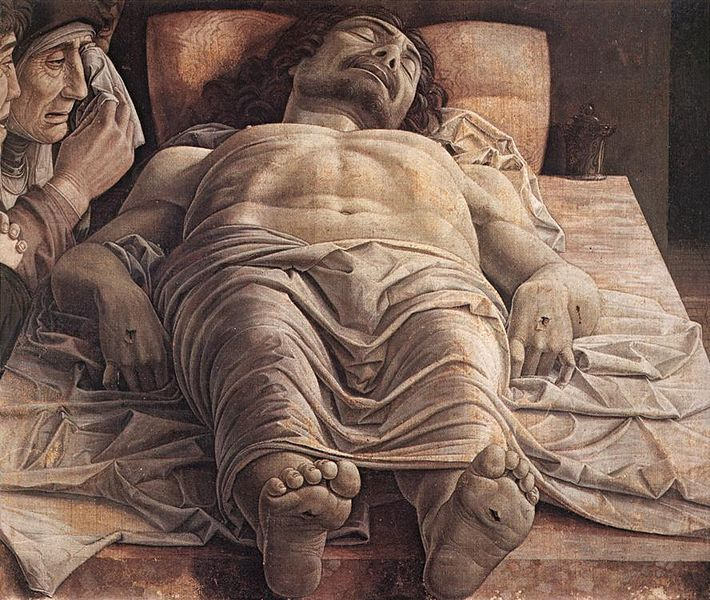
\includegraphics[width=\textwidth]{mantegna.jpg}
   .\caption{Lamentación sobre Cristo muerto de Andrea Mantegna. Pinacoteca de Brera.} % URL: smcarq.blogspot.com.es/2011/07/andrea-mantegna-lamentacion-sobre.html}
\end{figure}

\newpage

%Arte, estilo: Renacimiento italiano, quattrocento
%Cronología: 1480
%Lugar: Pinacoteca de Brera, Milán
%Autor: Andrea Mantegna
%Título: Lamentación sobre Cristo muerto
\begin{description}
\item[Estilo] Renacimiento italiano, Quattrocento
\item[Cronología] 1480
\item[Lugar] Pinacoteca de Brera, Milán
\item[Autor] Andrea Mantegna
\item[Título] Lamentación sobre Cristo muerto
\end{description}

%Función:
\textbf{Contexto histórico:}

Andrea Mantegna realizó esta obra en pleno período humanista, el centro del mundo ya no era Dios o la religión como anteriormente, sino que el hombre pasa a ser el centro. Este pensamiento derivaría en ideas de libertad, rivalidad, competencia, que no hacieron otra cosa que contribuir al gran avance que se dio en el arte durante el Renacimiento en general.

Fue en esta época cuando los pintores comienzan a tomar importancia como artistas, no solamente como meros técnicos. A partir de este momento empezaron a estudiar formas de hacer las obras más cercanas y reales para el espectador, otorgando especial importancia a la figura humana donde se buscaba la consecución de una imagen con volumen, profundidad y dimensiones adecuadas. De esta manera se dieron verdaderos progresos en la perspectiva, en las proporciones y en la anatomía humana.

La obra analizada fue, de hecho, una obra pionera en la perspectiva con la que representa a Cristo muerto. En épocas anteriores y en otras obras de la misma época en las que se representa a Cristo muerto, lo corriente era contemplarlo de perfil.

%TODO Dividir la frase del párrafo en más frases... Es larguísima!
Se trata de una obra dramática del cuerpo de Cristo muerto, antes de la resurrección y el triunfo sobre la muerte. Este dramatismo se percibe en la expresión tanto de la cara de la figura principal, como los rostros de aquellos que contemplan con horror la escena. Y se incrementa con los colores utilizados, de la misma gama cromática y la austera decoración del resto de la estancia, en la que solo vemos la lápida en la que se encuentra tumbado Cristo y la almohada en la que apoya la cabeza.

Además, en la búsqueda de realismo en su obra el autor ladea la cabeza y los pies de la figura, eliminando, de esta forma, la estaticidad que le aporta la simetría del cuerpo. Ésta también se ve disminuida mediante las arrugas de tela que cubren la pelvis y las piernas de Cristo y las formas laxas del cuerpo.

%http://www.arteespana.com/quattrocentoitaliano.htm
%http://www.arteespana.com/andreamantegna.htm
%http://www.artehistoria.jcyl.es/v2/obras/4376.htm
%http://educacion.ufm.edu/andrea-mantegna-lamentacion-sobre-cristo-muerto-oleo-sobre-tela-en-torno-a-1480-1490/
%http://cv.uoc.edu/~04_999_01_u07/percepcions/perc57.html
%Libro de Olatz


\vspace{12pt}
\textbf{Anatomía de superficie:}

Andrea Mantegna sorprende en su época con esta obra en la que Cristo se presenta en una perspectiva nunca antes vista, y con una figura de proporciones y anatomía exquisitas. Debido precisamente a la perspectiva en la que se encuentra la figura no es fácil discernir el modelo proporcional que sigue, aunque si es apreciable la armonía en la proporción de la figura, con una cabeza adecuada al tamaño del resto del cuerpo.

En esta obra se aprecia de manera sublime la muerte de Cristo. La laxitud de los músculos de las extremidades y la lividez que presenta el cuerpo nos da una idea bastante acertada de la imagen de un cadáver. La palidez amarillenta con la que el autor refleja el cuerpo y los tonos grisáceos incluso amoratados hacen visible lo que se denomina el \textit{pallor mortis}. Esta es una de las fases que acontece a nuestro cuerpo una vez el corazón deja de bombear sangre y, por tanto, esta no llega a los capilares, produciendo una palidez cadavérica. Una vez la sangre deja de circular tiende a por gravedad a dirigirse a la parte baja del cuerpo, que en el caso de la figura de la obra sería en su zona dorsal. En la obra se aprecian zonas más oscuras que podrían coincidir con estas zonas amoratadas del \textit{livor mortis}, pero podrían, de igual manera, tratarse de la propia sombra que proyecta la figura.

Se contemplan los orificios creados por los clavos en primer plano, tanto en los pies como en las manos, representados con gran realismo por el autor. Se pueden observar estos según las creencias de la época en las palmas de las manos, en lugar de a la altura de las muñecas, donde de acuerdo con la creencia actual, eran introducidos.
Las heridas, tanto las originadas por los clavos como la producida por la lanza, se encuentran limpias y sin una gota de sangre. Tanto es así que la del costado derecho apenas es visible en la perspectiva de la figura.

Se puede apreciar sin esfuerzo el volumen de las distintas partes del cuerpo que el autor plasma duramente, casi a modo escultórico. 

Se percibe la distensión de todos los músculos del cuerpo muerto, pudiendo, además, observar estructuras que en obras tan antiguas no solían aparecer, como son las plantas de los pies, donde apreciamos diversas estructuras anatómicas: el arco plantar, claramente definido y el calcáneo y las cabezas de los metatarsianos, que están cubiertos por grasa subcutánea que sirve de almohadillamiento.

También se perfila de forma aparente la caja torácica, tras un vientre hundido, que hace notable el borde costal inferior. Y aunque las estructuras no están claramente representadas se puede intuir, debido al vientre hundido, la espina ilíaca en ambos costados de la pelvis.

Además de estructuras óseas se observan ciertos músculos que recubren tanto la cavidad abdominal como la torácica.

En la porción abdominal, se encuentra, aunque no muy definido, el músculo recto del abdomen y el oblicuo externo, que es el músculo más superficial de los músculos laminares.

En la porción torácica el autor refleja los músculos pectorales y superficialmente incluso identifica los pezones. Sin embargo, da la sensación de que estos músculos tienen la inserción humeral más distal de lo anatómicamente preciso teniendo en cuenta que en realidad insertan cerca de la epífisis del húmero, formando simplemente, el pliegue axilar anterior. Esta sensación puede ser debida a un problema de perspectiva. Otro defecto que podemos observar en la anatomía de este Cristo fallecido es la posición de los hombros con respecto al tronco, estando más ``caídos" de lo que podríamos ver a una persona en la misma posición y desde la misma perspectiva, dejando a la vista un torax en apariencia hinchado. Este tórax hinchado no podría deberse al estado de descomposición en el que se encuentra la figura, puesto que la hinchazón del cuerpo causada por los gases producidos por las bacterias que se encuentran en éste se produce en un estado más avanzado de descomposición.

Las extremidades superiores caen inertes a ambos lados de la figura, con cierta flexión en las articulaciones del codo, muñeca, metacarpofalángicas e interfalángicas probablemente debido al \textit{rigor mortis}. Éste se define como la rigidez que adquieren los músculos tras varias horas de la muerte debido a cambios químicos en las células del cuerpo. Refiriéndome a este mismo proceso, he de mencionar la rigidez de las piernas, puesto que si tal caso no se diera los pies caerían laxos hacia los lados. El músculo deltoides se puede vislumbrar en todo su esplendor recubriendo la articulación del hombro, pero su delimitación es demasiado firme, pudiendo apreciar claramente donde finaliza éste.

%\section{Análisis de la obra pictórica: Cristo crucificado de El Greco}

\begin{figure}[ht!]
    \centering
    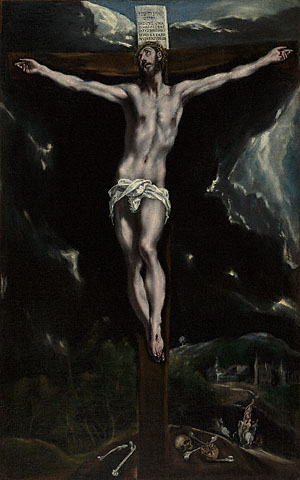
\includegraphics[width=0.9\textwidth]{elgreco.jpg}
   .\caption{Cristo crucificado de El Greco. Museo J. Paul Getty.} % URL: www.getty.edu/art/gettyguide/artObjectDetails?artobj=138292\&handle=li}
\end{figure}

\newpage

%Arte, estilo: Manierismo
%Cronología: Hacia 1600-1610
%Lugar: Museo J. Paul Getty, Los Ángeles
%Autor: El Greco
%Título: Cristo crucificado 

%Función: Purchased by a Spanish family at a flea market around 1950, it remained in their possession until recently. 
% http://www.ctv.es/USERS/ags/00013_mm.htm
% http://www.google.com/culturalinstitute/asset-viewer/christ-on-the-cross/cgHO8uo2dVOJoQ?hl=es&projectId=art-project


\begin{description}
\item[Estilo] Manierismo
\item[Cronología] Hacia 1600-1610
\item[Lugar] Museo J. Paul Getty, Los Ángeles
\item[Autor] Doménikos Theotokópoulos, más conocido como el Greco
\item[Título] Cristo crucificado
\end{description}

\textbf{Contexto histórico:}

El cuadro se realizó en plena contrarreforma. Durante este período la Iglesia católica intentaba consolidar su poder bajo la amenaza de la reforma protestante, es por eso que durante esta época se produjeron un gran número de obras de contenido religioso. De hecho la gran mayoría de las obras elaboradas por el Greco son de naturaleza religiosa, centrándose menos en retratos u otro estilo de obras. La obra a analizar es una de estas obras de carácter religioso.

En esta, y en general en todas sus obras, el Greco utilizaba un estilo propio basándose en el estilo veneciano en el uso del color y en el Manierismo alargando y retorciendo las formas y figuras. Dejó, de esta forma a un lado el orden, la claridad, la proporción y el equilibrio característico del Renacimiento anterior.

Se observan grandes contrastes en el uso del color en esta obra. Las figuras parecen emanar luz propia, pues están envueltas en oscuridad y exclusivamente hay luz en las formas que el autor quería que advirtiésemos. Además, esta utilización del color nos lleva a discernir la sombría situación del calvario de Cristo.

El alargamiento de las formas, propio de el Greco, provee a la obra de mayor belleza y misticismo, lo que le valió el reconocimiento de muchos religiosos de la época.

Siguiendo el estilo de su época el Greco representó la crucifixión de Cristo mediante tres clavos: un clavo que junta ambos pies a la cruz directamente y un clavo en cada palma de la mano, según la interpretación bíblica de la época, contrariamente a la creencia actual principal de que se encontraban a la altura de las muñecas.


\vspace{12pt}
\textbf{Anatomía de superficie:}

En esta obra el Greco nos muestra un Cristo que presenta una anatomía adecuada excepto en sus proporciones. La figura sigue una proporción de nueve cabezas, pudiendo apreciar, efectivamente la cabeza pequeña de la figura mientras el tronco y sus extremidades son extremadamente alargados, no concordando con ningún cánon de proporciones habitual \footnote{Actualmente existen tres cánones para determinar las proporciones de la figura humana: el cánon de siete cabezas y media, el cánon más relista en cuanto a medidas, que se considera la figura común, el cánon de ocho cabezas considerado la figura ideal y el cánon de ocho cabezas y media, con el que se representan las figuras heróicas.}. Sin embargo estas medidas dotan a la figura de una mayor heroicidad, presentando de esta forma, y junto con otros detalles de la obra, el triunfo de Cristo sobre la muerte, idea que en la contrarreforma querían destacar. Su longitud con los brazos extendidos es igual a su altura y el ángulo que forman entre ellos es de 135º.

Como la figura no ha fallecido no es posible observar las características típicas de la muerte como es la lividez del cuerpo o la laxitud muscular. Es más, la figura conserva los ojos abiertos, mostrando una ausencia de sufrimiento en el rostro, lo que es otro detalle de la obra en la que se ilustra el triunfo de Cristo, que inexpresivo mira al cielo (a Dios) a la espera de su muerte. La posición retorcida del cuerpo es utilizada por el autor para aumentar la belleza del cuadro, sin reparar en que es extremadamente difícil adquirir esa posición estando crucificado y al borde de la muerte. Tanto los músculos de los brazos como los de las piernas que contribuyen al mantenimiento de la postura están contraídos y extendidos, sin embargo los de la espalda, muy necesarios para el mantenimiento de esta postura no se observan claramente.

Apoya la mayor parte del peso del cuerpo sobre la pierna derecha aprovechando para inclinar la cadera hacia el mismo lado produciendo la curvatura del cuerpo de la que he hablado anteriormente y que se continuará en forma de \textit{S} a lo largo de la figura.

Además, existen otros signos que muestran el triunfo de la vida sobre la muerte. Uno de ellos es la escasa sangre que se visualiza en este cuadro, quitando de esta manera importancia a las heridas de la carne y dando una apariencia más divina. No encontramos la herida del costado derecho, lo que, de hecho, es lógico debido a que esta se le ocasiona después de morir, para verificar su muerte.

Para conseguir la postura que mantiene la figura intervienen varios músculos.
Tanto la espalda como el cuello se encuentran en posición erguida, con el rostro mirando hacia arriba, utilizando para ello los músculos erectores de la columna: los músculos del grupo iliocostal, los del grupo longuísimo y los del espinoso y los principales músculos del cuello como el esplenio y el esternocleidomastoideo, este último visible en la obra. Otro músculo que participa en la postura erecta es el recto del abdomen, el cual se puede discernir en la obra, junto con la línea alba, formada por la unión de vainas fibrosas en la línea media, y la línea semilunar, que marca el borde lateral del músculo recto del abdomen.

El músculo dorsal ancho que proviene de la espalda posee un tendón estrecho que envuelve al músculo redondo mayor formando el pliegue posterior de la axila, reconocible en esta imagen. Estos músculos producen la elevación del tronco estando los brazos fijos, por tanto tienen gran relevancia en la crucifixión. Además de estos dos músculos otro que participa en la elevación del tronco es el pectoral mayor que forma el pliegue anterior de la axila, también visible en la obra.

Otros músculos con gran relevancia en esta posición son: el trapecio, que se puede observar en la figura, y el elevador de la escápula, que elevan la escápula, y el serrato anterior que la gira. La posicion de Cristo en la cruz desplaza la escápula de esta forma.

El músculo deltoides se aprecia sin esfuerzo rodeando la articulación de los hombros en ambas extremidades superiores. Su principal función es la abducción del brazo y es por eso que se le confiere gran importancia en la posición en la que ambos brazos están en abducción.

En el brazo, aunque no con trazos muy firmes, son evidentes los músculos bíceps y tríceps. El primero se encuentra en la parte anterior del brazo y su principal función es la flexión de la articulación del codo, sin embargo en esta figura los brazos se encuentran en extensión por la que la función principal del bíceps no es la anteriormente citada sino la supinación del antebrazo, la cual la realiza junto con el músculo supinador. Por su parte el tríceps se encuentra en la parte posterior siendo su principal función la extensión de la articulación del codo, lo que posee importancia en esta posición. 

Las manos se encuentran en posición de reposo, por lo que el tercer, cuarto y quinto dedo se encuentran ligeramente flexionados, no siendo así, sin embargo, en el primer y el segundo dedo que se encuentran extendidos, posiblemente debidos a los clavos con los que se sujeta a la figura en la cruz. Estos no están representados en el centro de las palmas de las manos, como era habitual, si no que se sitúan entre los segundos y terceros huesos metacarpianos.

La caja torácica es fácilmente visible: el borde costal inferior, la depresión en la que se encuentra el esternón, algunas costillas (probablemente la tercera y la cuarta) e, incluso, ambas clavículas elevadas debido a la elevación de los brazos, que a su vez hace posible la óptima visualización de las estructuras anteriormente citadas. Igualmente, como el autor de la obra representa a un Cristo más bien delgado, la espina ilíaca puede ser divisada superficialmente en ambos lados de la pelvis.

La extremidad inferior izquierda mantiene la articulación de la rodilla ligeramente flexionada, mientras que la derecha la mantiene totalmente extendida. A su vez la cadera se encuentra ladeada hacia el lado de la pierna estirada, provocando que la espina ilíaca sea más fácilmente visible en este costado que en el izquierdo.
Los encargados de mantener esta postura son: en la extensión, el cuadriceps y los músculos del tracto iliotibial, y en la flexión, los músculos poplíteos y los gemelos. La rótula o patella, que se encuentra en la articulación de la rodilla se vislumbra perfectamente junto con la tuberosidad tibial en la rodilla flexionada. Aún así, la tuberosidad tibial, anatómicamente recta desde la articulación de la rodilla hasta la articulación del tobillo, se presenta curvada en el afán de el Greco por moldear las formas a su antojo

Los pies se encuentran uno sobre otro,el izquierdo sobre el derecho, y ambos clavados juntos en la cruz. Mantienen el peso de la mayor parte del cuerpo, ayudados por los músculos que elevan el tronco y los clavos que sujetan ambos brazos.
\section{Análisis de la obra pictórica: Cristo crucificado de Velázquez } 

Arte, estilo: Barroco

Cronología: 1632

Lugar: Museo del Prado, Madrid,España

Autor: Diego Velázquez

Título: Cristo crucificado

Función: Aunque se encontraba en el Convento de la encarnación de San Plácido, no está claro donde estuvo los primeros años tras su realización ni la función específica que desarrollaba. Posteriormente se tiene constancia de que estuvo en la sacristía de este convento hasta alrededor del 1804, año en el que Godoy lo compra al convento. Pasa después por distintas manos, llegando finalmente al Museo de Prado en 1829, donde permanece actualmente. % El Cristo crucificado de velazquez, trasfondo histórico religioso. % http://www.museodelprado.es/coleccion/galeria-on-line/galeria-on-line/obra/cristo-crucificado-1/

\textbf{Anatomía de superficie}
En esta obra Velázquez nos cautiva con una figura con una postura serena y de proporciones y anatomía estudiadas. Responde a un modelo de siete cabezas y media. Su longitud con los brazos extendidos es igual a su altura y el ángulo que forman entre ellos es de 113º. La cadera esta ligeramente inclinada hacia el lado derecho, dando la sensación de apoyo del peso en el lado izquierdo, lo que se podría interpretar como un ligerísimo contrapposto clásico.
En el cuadro se puede observar la parte izquierda de la cara, la parte derecha está cubierta por el cabello que cae sobre ella. En cuanto a aquello que podemos ver, se trata de una cara inexpresiva con barba que cubre parte de las mejillas y el mentón. Bajo esta barba se puede apreciar la forma del hueso de la manbíbula (cuerpo, rama y ángulo). La mucosa de los labios es apenas visible entre el vello, aunque sí se intuyen incluso la comisura labial izquierda. La nariz se presenta en el centro de la cara de forma piramidal. La estructura de la nariz la proporcionan los huesos nasales que articulan entre sí, con el hueso frontal(por donde se une a la frente) y con el hueso maxilar (por el que se une  a las mejillas). La parte más prominente de la nariz es el cartílago nasal que separa las dos fosas nasales. Se aprecia el espacio del surco naso-labial, aunque éste no se ve directamente, porque al igual que el mentón, está cubierto de vello. Sin embargo, sí se distingue la aleta nasal izquierda y el septo nasal, a la vez que se puede intuir la narina izquierda de la nariz. Se puede también vislumbrar una pequeña arruga, la línea naso-labial. Se puede ver la prominencia de la mejilla, formada por el hueso cigomático. Entre la nariz y la frente se encuentra una depresión denominada nasión. La frente, formada por la convexidad lisa del hueso frontal, apenas es visible puesto que está tapada por la corona de espinas. Sus bordes inferiores (arcos supraciliares) dan lugar al borde superior de cada órbita. Además estos dos arcos se unen mediante un puente denomindo gabela. Superficialmente a estas elevaciones se encuentran las cejas. Medialmente el globo ocular está limitado por los huesos maxilar y frontal que articulan entre ellos, lateralmente está limitado por los huesos frontal y cigomático e inferiormente por el hueso maxilar. El globo ocular izquierdo no es visible, solo se adivina debajo del párpado superior que lo cubre, en el que además se puede observar una pequeña arruga. Sí se puede vislumbrar las uniones medial y lateral entre los párpados superior e inferior, que limitarían la hendidura palpebral en caso de estar abiertos. En sus bordes se encuentran las pestañas, manifestadas en la obra mediante una línea más oscura en el borde de los párpados. Ambas orejas están tapadas por el cabello, por lo que sus partes no son visibles.
El resto de la cabeza está formada por la bóveda craneal, la cual se insinua debajo del cabello. La cara lateral de la bóveda la componen los huesos frontal, parietal, occipital y temporal.
El cuello no es visible, al estar la cabeza caída hacia abajo, ésta tapa las estructuras anatómicas del cuello.

En la imagen se puede observar el torso desnudo de Cristo crucificado, en el que se aprecian una serie de estructuras anatómicas. 

Al tratarse de un individuo delgado se puede intuir la caja torácico perfectamente. Vislumbramos, a duras penas, la clavícula izquierda que articula con el esternón (manubrio) y la primera costilla, la derecha, no es visible, puesto que está tapada por el cabello. El borde costal inferior formado por las seis últimas costillas es fácilmente visible, al igual que la depresión en la que se encuentra el cuerpo del esternón y el contorno de algunas costillas (probablemente la cuarta, quinta, sexta y séptima), sobre todo las del lado derecho, ya que la sombra del propio cuadro nos  impide ver bien las del izquierdo. La escotadura esternal, también se puede intuir sobre la cara superior del manubrio, sin embargo, hay que dejarse llevar un poco por la imaginación, ya que, de nuevo la sombra del cuadro nos impide su correcta visualización. No se observa la apófisis xifoides, que está cubierta, por el recto anterior del abdomen, lo que se considera normal.

En cuanto a los músculos podemos vislumbrar el pectoral mayor, que inserta en el borde interno de la clavícula, en los cartílagos de las seis costillas superiores y en el húmero, formando así el pliegue anterior de la axila, muy claro en la imagen, junto con el músculo deltoides, que se puede contemplar recubriendo la articulación del hombro. Lateralmente no se observan claramente los músculos. El serrato anterior que inserta en el borde anterior interno de la escápula, y en las ocho costillas superiores, junto con sus interdigitaciones con el músculo oblicuo externo podrían ser visibles en un individuo delgado y musculoso como el Cristo que representa este cuadro, sin embargo no es fácil de reconocer. Sí se puede apreciar el músculo dorsal ancho, proveniente de la espalda e insertado en el ángulo inferior de la escápula. Su tendón estrecho envuelve al músculo redondo mayor que forma el pliegue posterior de la axila. Este va desde el borde lateral de la escápula hasta el surco bicipital del húmero. El borde lateral de la escápula puede percibirse a través de la masa del redondo mayor.
Los pezones se encuentran en el Cristo de la obra alrededor del cuarto espacio intercostal, lo que es anatómicamente correcto.

En el abdomen, que delimita superiormente con el reborde costal, que como ya he dicho es claramente visible en esta obra, se encuentran los músculos abdominales, que se pueden apreciar, aunque no muy marcados. Estos músculos forman una vaina fibrosa a cada lado de la línea media que se unen en esta, formando la línea alba. La figura no está suficientemente musculada para poder apreciar las tres inserciones tendinosas que se encontrarían encima del ombligo, a duras penas podríamos localizar una de ellas. Sí se divisa bastante bien la línea semilunar, que marca el borde lateral del músculo recto del abdomen. La espina ilíaca si se aprecia, sobre todo en el lado derecho, que es el lado hacia el que está ligeramente inclinada la cadera.
El músculo mas superficial de los músculos laminares del abdomen es el oblicuo externo , pero como ya he comentado anteriormente no se ve claramente, y aunque sepamos que tiene que estar ahí, sus interdigitaciones con el serrato anerior no son visibles en el cuadro. Este músculo se inserta superiormente en las ocho costillas inferiores e inferiormente en la sínfisis de púbis, tuberosidad púbica, espina ilíaca anterosuperior y cresta ilíaca. Entre la espina y la tuberosidad púbica gira sobre sí mismo y forma el ligamento inguinal. La depresión que suele haber a la altura de ese ligamento, y que suele ser más visible en hombre, se puede observar perfectamente en la obra pictórica.
Las estructuras pélvicas no son visibles, debido a que el autor coloca encima un paño blanco con el que las tapa.

Las extemidades superiores se encuentran extendidas cada una hacia un costado de la cruz: Los músculos son visibles claramente. Antes de empezar con los músculos del brazo propiamente dichos, remarcaré algúno que se encuentra sustentando la articulación del hombro. El múculo trapecio sí se observa, este lateralmente se inserta en el tercio externo de la clavícula, el acromion y la espina de la escápula. Estas estructuras no son visibles anteriormente en la posición en la que se encuentra la figura analizada (brazos extendidos hacia los lados), sin embardo podemos apreciar un hueco en la unión de este músculo a las estructuras previamente citadas. El músculo que no nos deja ver esas estructuras es el deltoides, que también se ve fácilmente redondeando la articulación del hombro por su parte superior, cubriendo la epífisis proximal del húmero. Se inserta medialmente, al igual que el trapecio, en la clavícula, el acromion y la espina de la escápula y lateralmente en el tubérculo deltoideo de la cara lateral del húmero. Es el principal abductor del brazo por lo que tiene gran relevancia en esta posición.
En el brazo se observan tanto el bíceps como el tríceps. El bíceps forma una prominencia en la parte anterior del brazo. Tiene dos cabezas, de las cuales la corta inserta en la apófisis coracoides y la larga en la cara superior de la fosa glenoidea de la escápula. Distalmente se inserta en la tuberosidad bicipital del radio, pasando por el medio de la fosa cubital.
En ambos brazos podemos distinguir la fosa cubital. Esta está limitada superiormete por la línea que va desde la epitróclea hasta el epicóndilo del húmero, lateralmente por el músculo braquiorradial y medialmente por el pronador redondo.
Los huesos de la articulación del codo suelen ser evidentes. En esta obra no se pueden distinguir claramente las distintas estructuras debido a la posición de los brazos (se verían mejor desde la cara posterior). Lo único que se aprecia de forma clara es la epitróclea del húmero.
Los brazos se encuentran en total supinación y extensión. La extensión la realiza el tríceps junto con la contribución de los músculos del origen del extensor común. Y de la supinación se encargan el bíceps y el supinador.

A la altura de las muñecas podemos observar las apófisis estiloides del cúbito y del radio, que en una persona un poco más gruesa no serían visibles. Además, se podrían intuir los tendones de los músculos del antebrazo que pasan a la mano. Cuando se flexiona la muñeca sobresalen tres tendones. El flexor carpi raialis se inserta distalmente en la base de los metacarpos 2 y 3, el flexor carpi ulnaris de inserta en el pisiforme y de allí en el ganchoso y en la base del quinto metacarpiano.
Las venas, tanto cefálica como basílica suelen se visibles en mayor o menor medida en hombres jóvenes, delgados y en cierta medida musculados, no obstante, no han sido dibujadas por el artista en esta figura.
En la obra se puede apreciar la palma de la mano derecha, aunque parcialmente, pues en ella se encuentra clavado el clavo a la cruz y, además los dedos se encuentran ligeramente flexionados, por lo que podemos vislumbrar las articulaciones interfalángicas en ellos. El metacarpiano del primer dedo también lo podemos distinguir en el cuadro. Este posee más movilidad que el resto de los metacarpianos, que además no son visibles en el cuadro, puesto que están tapados por los músculos de la palma.
En la mano izquierda básicamente se observan las mismas estructuras que en la derecha. Pero además podemos percibir la denominada tabaquera anatómica. La tabaquera anatómica es una concavidad presente en la cara lateral de la muñeca, que se evidencia más al extender el primer dedo. Está limitada por varios tendones: el abductor largo del pulgar, que se inserta distal al primer metacarpiano; el extensor corto del pulgar, que se inserta en la falange proximal del pulgar; y el extensor largo del pulgar, que inserta en la falange distal del primer dedo.
En las palmas de ambas manos se observan tanto la eminencia tenar, como la hipotenar.
La emnencia tenar se denomina al abultamiento lateral presente en la palma de la mano, a la altura del primer dedo. Está formada por los músculos cortos del pulgar: los músculos abductor, flexor y oponente del pulgar.
La eminencia hipotenar se denomina al abultamiento medial de la palma de la mano a la altura del quinto metecarpiano. Está formada por el abductor, el flexor y el oponente del meñique.
Podemos apreciar cierta flexión en las articulaciones metacarpofalángicas, la cual es producida por los músculos lumbricales que se encuentran entre los dedos. Los dedos también mantienen cierta flexión, producida esta por los tendones de los flexores superficial y profundo de los dedos.
\subsubsection{Visión anterior del antebrazo}
El músculo pronador se inserta sobre la cara anterior de la epitróclea y en la región central del radio. Es un pronador del antebrazo. Los tendones de los músculos flexor carpi radialis, palmar mayor, flexor superficial de los dedos y flexor carpi ulnaris pasan a la mano. Son también flexores débiles del codo.
El músculo braquiorradial se inserta proximalmente  en los dos tercios superiores de la cresta supracondílea del húmero y distalmete en la cara lateral de la epífisis distal del radio. Este músculo prona o supina el antebrazo.

El pisiforme es visible, así como el tubérculo del escafoides.

Podemos apreciar claramente la masa muscular de las estremidades inferiores, ya que estas se encuentran al descubierto. Sin embargo no es así de fácil distinguir los músculos específicos que producen esta masa muscular.
Podemos intuir a duras penas por donde pasa el músculo sartorio, que que inserta en la espina ilíaca y en la superficie subcutánea medial de la parte superior de la tibia. Así mismo se podría señalar el músculo cuadriceps, músculo principal de la cara anterior del muslo, junto con sus tres cabezas superficiales: vasto externo, vasto interno y recto anterior, no el vasto intermedio, que va bajo el recto anterior. Los músculos pectíneo, psoas-ilíaco y recto interno no son visibles pues están tapados por el paño blanco que también tapa las estructuras pélvicas. No son claramente apreciables otros músculos superficiales como el tensor de la fascia lata (que inserta en la cara externa del ilion y en la tibia, formando el tracto iliotibial al unirse con el glúteo mayor), que esta situado en el lateral del muslo, superficialmente al trocánter mayor del fémur.
El músculo cuadriceps forma en su parte inferior el "ligamento patelar" que recubre la rótula y se inserta en la tuberosidad tibial. En una figura delgada como esta la rótula o patella se puede apreciar, al igual que la tuberosidad tibial, aunque son más fáciles de apreciar en la flexión de la rodilla.
El resto de estructuras de la rodilla no son apreciables, aunque se pueden intuir: condilos femorales, ligamentos de la articulación, tubérculo adductor del fémur, retináculos rotulianos medial y lateral...
Las articulaciones de las rodillas de la figura se encuentran una en posición de extensión,mientras que la ptra se encuentra ligeramente flexionada. Los músculos encargados de la extensión son: el cuadriceps y los músculos del tracto iliotibial, y los de la flexión son: los músculos poplíteos y los gemelos.
Podemos apreciar la tibia desde latuberosidad tibial hasta el maleolo medial, en su recorrido subcutáneo.
La masa muscular que se puede visualizar la conforman varios músculos. El músculo tibial anterior se encuentra en el lateral de la pierna y es el único de los cuatro músculos que inserta en la tibia. Además tiene un tendón distal que pasa hacia la base del primer metatarsiano. Otros músculos que forman esta masa muscular son el extensor largo del dedo gordo y el extensor largo de los dedos. Sin embargo también se pueden apreciar en la cara lateral músculos que en principio forman parte de la parte posterior: el sóleo y una de las cabezas del gemelo (superior al sóleo), que se unen para formar el comunmente denominado tendón de aquiles. Más lateral se encuentra el músculo peroneus tertius.
A la altura de la articulación del tobillo se pueden contemplar ambos maleolos, interno formado por la tibia y externo formado por el peroné (que en el resto de su recorrido por la pierna está rodeado por músculos). Anatómicamente el maleolo externo se encuentra un centímetro más abajo que el maleolo interno. En la representación pictórica se reproduce correctamente esta característica.

Al estar de pie sobre una pierna el lado de la pelvis que no soporta peso se eleva para evitar que la pierna libre no pise el suelo. Esta acción está realizada por los glúteos medio y menor.

Los pies se encuentran apoyados en una tabla,lo que permite que sus rodillas y cadera estén ligeramente flexionadas. Apoyados sobre el hueso calcáneo y la articulación metatarsofalángica, cuya prominencia es visible bajo la grasa subcutánea que sirve de almohadilla, dejan intuir claramente el arco plantar, mantenido por los músculos cortos y los tendones del flexor largo. Los pies se ubican en paralelo entre ellos ligeramente suparados aneriormente, con un clavo en cada dorso y sangre que emana de la herida, lo que nos hace más dificil la visión de las estructuras que se encuentran en el dorso del pie. La cara lateral es peor visible, debido a la gran dfuminación de los colores en esta zona y a la oscuridad con la que el artista simula la sombra de la figura. Más medialmente se pueden observar tendones (del músculo extensor largo de los dedos, del músculo extensor largo del dedo gordo y de los músculos peroneos) y prominencias óseas que no son claramente distinguibles. En la parte anterior, los dedos se encuentran relajados y las uñas nacen de cada uno de ellos superficialmente.
El extensor corto de los dedos es el único músculo situado en el dorso del pie y se extiende desde el hueso calcáneo. Sus tendones se insertan en la falange proximal del primer dedo y en la cara lateral de los tendones del extensor de los dedos segundo, tercero y cuarto.

La cara posteromedial del calcáneo, el sustentaculum tali, el tubérculo del navicular.


Colores: primarios, secundarios, fríos, cálidos, paleta de colores.

Línea, dibujo

Luz

Perspectiva

Movimiento o quietud

Proporciones

Iconografía

Resolución del tema

Momento de la narración elegido

\section{Análisis de la obra pictórica: Cristo de San Juan de la Cruz de Dalí}

\begin{figure}[ht!]
    \centering
    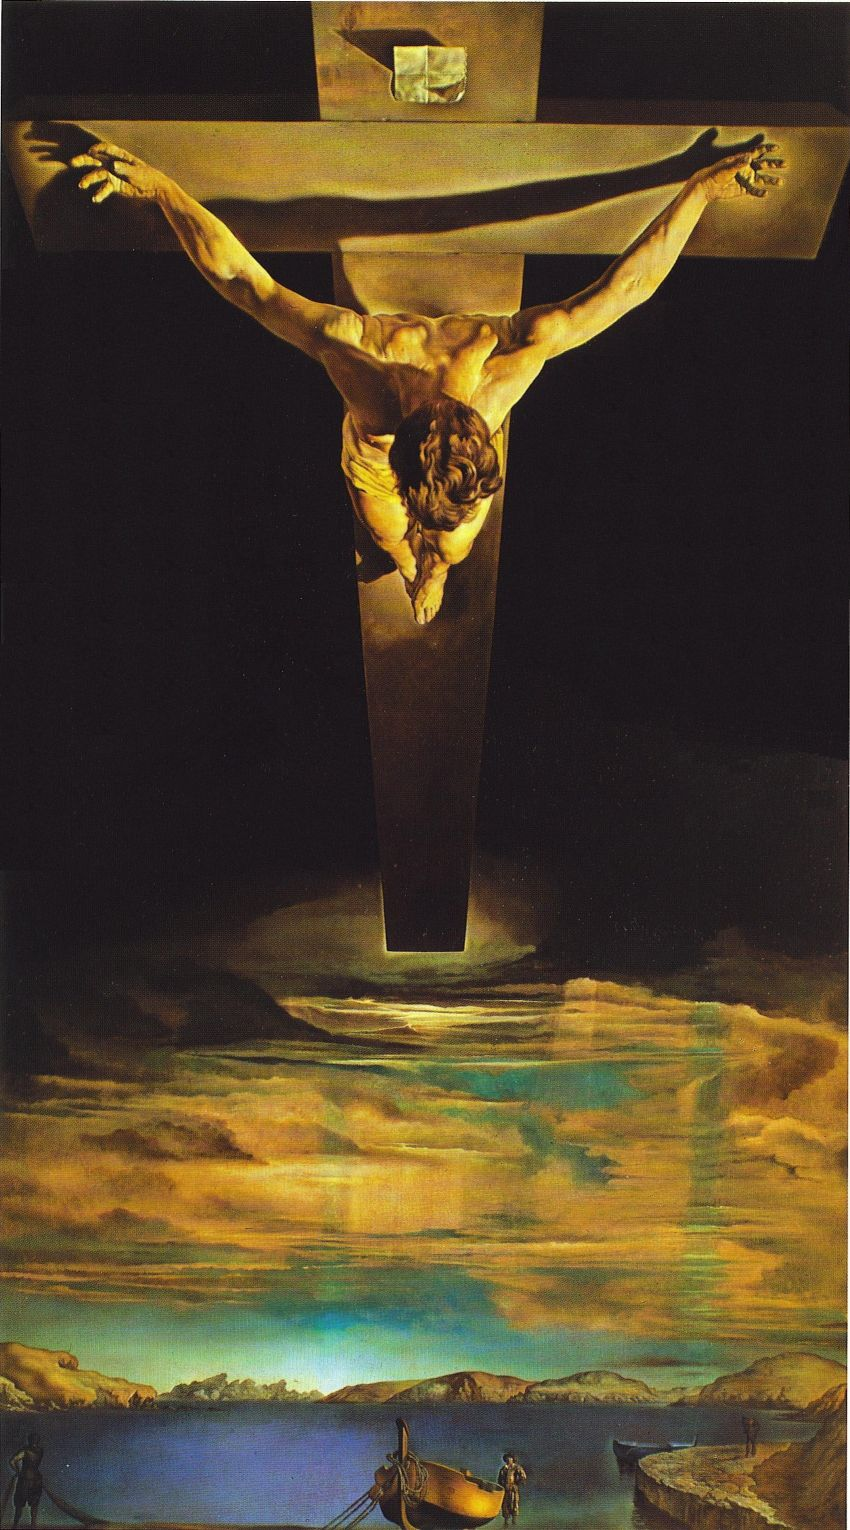
\includegraphics[width=0.84\textwidth]{dali.jpg}
   .\caption{Cristo de San Juan de la Cruz de Salvador Dalí. Museo Kelvingrove.} % URL: blogsantiagosoul.wordpress.com/tag/viva-la-vida}
\end{figure}

\newpage

%Arte, estilo: Surrealismo
%Cronología: 1951
%Lugar: Museo Kelvingrove, Glasgow, Reino Unido
%Autor: Salvador Dalí
%Título: Cristo de San Juan de la Cruz

%Función: Se expuso por primera vez en la galería Lefevre de Londres. %http://www.xn--esarteespaol-jhb.es/contenido.php?recordID=11

\begin{description}
\item[Estilo] Surrealismo
\item[Cronología] 1951
\item[Lugar] Museo Kelvingrove, Glasgow
\item[Autor] Salvador Dalí
\item[Título] Cristo de San Juan de la Cruz
\end{description}

\textbf{Contexto histórico:}

Esta obra se realizó en plena dictadura franquista, en la que numerosos artistas fueron desterrados por no compartir las ideas de la dictadura. No siendo así para Dalí que no sólo aceptó la dictadura franquista, sino que incluso elaboró un retrato de la nieta del propio Franco.

Gran pintor de estilo surrealista, Dalí siguió un estilo propio y más extravagante que el del resto de sus compañeros. El surrealismo nació en 1924, en París a manos de André Breton que publicó el \textit{Primer Manifiesto Surrealista}. Los pintores de esta corriente, influidos enormemente por las teorías de Freud, intentaron expresar en sus obras el mundo del subconsciente.

Dalí enseguida sobresalió en este estilo con una primera etapa más agresiva. Sin embargo, a partir del 1948, cuando regresó a Europa de América, inició una etapa en la que vuelve al clasicismo, reproduciendo sus primeros temas religiosos. Una de estas obras religiosas es la del Cristo de San Juan de la Cruz. Este Cristo está basado, como su nombre indica, en el Cristo dibujado por San Juan de la Cruz tras una revelación.

Dalí decidió representar \textit{un Cristo bello como el mismo Dios que él encarna} y no centrase en la fealdad para provocar la emoción en el espectador. Lo hizo adoptando una perspectiva totalmente nueva de la crucifixión. Con este nuevo enfoque situó a Cristo en la Cruz en una posición vertical y casi perpendicular al espectador de la obra.

Además decidió retirar todos aquellos elementos que intervinieron en la crucifixión de Cristo, nótese que éste no conserva la corona de espinas ni ninguna herida, tampoco están dibujados los clavos que lo deberían sostener en la cruz, en la que parece que está suspendido por arte de magia.

Debajo de la imagen principal del cuadro se puede apreciar un paisaje, supuestamente representado a partir de la bahía de Port Lligat. En ella se ven dos pescadores que, sin embargo, están inspirados en los pintores Le Nain y Velazquez.

El Cristo se sitúa en un fondo oscuro que le da una imagen dramática a la obra junto al contraste con la iluminación que se proyecta en forma de rayo de luz sobre la figura. Entre la imagen del crucificado y la de los pescadores se interpone un cielo nuboso, que aporta a la obra aún mayor dramatismo al separar la crucifixión y la imagen de la tranquila bahía de pescadores, dando a entender la indiferencia de éstos ante el suceso que se está produciendo.

% http://www.artehistoria.jcyl.es/v2/obras/9639.htm
% http://unapizcadecmha.blogspot.com.es/2013/11/el-cristo-de-san-juan-de-la-cruz-1951.html
% http://www.arteespana.com/salvadordali.htm
% Artículo de San Juan de la Cruz
% libro de aita

\vspace{12pt}
\textbf{Anatomía de superficie:}

En esta obra en la que Dalí refleja una nueva perspectiva de la crucifixión de Cristo, siendo la cabeza de éste el centro de la obra, podemos observar un Cristo de con características totalmente diferentes a las apreciadas en la mayoría de obras acerca de la crucifixión. Aparte de tener el pelo corto, al contrario que en las numerosas obras en las que se representa a Cristo, no posee signos de sufrimiento, ni clavos que le sujeten a la cruz, ni corona de espinas, ni tampoco sangre puesto que no hay heridas de las que pueda brotar.

Aún sin elementos de crucifixión la figura mantiene una posición en la que se sugiere que ambos pies estarían unidos a la cruz mediante el mismo clavo, mientras que los clavos de las extremidades superiores se encontrarían en las palmas de las manos. Esto último se puede percibir en la caída del cuerpo hacia delante que ocurre desde más arriba de las muñecas, según la sombra que se proyecta detrás.

Al estar la cabeza inclinada hacia delante, no es posible ver el resto del cuerpo de la figura, sin embargo si ofrece una visión espectacular de la espalda y de sus músculos. Los brazos caen extendidos, formando un triángulo con la cruz que mantiene suspendido a Crsito y dando una sensación de que éste se encuentra colgado boca abajo por el espacio que hay entre su cuerpo y la cruz.

El autor en esta obra de arte no se centra en el sufrimiento y la muerte de Cristo, sino que intenta evocar la belleza de Cristo Dios. Por ello se puede considerar admirable la simetría del cuerpo y la anatomía que se vislumbra. La actitud de la figura es relajada, pudiéndose observar este hecho en la posición de sus brazos y de los músculos de la espalda.

No es posible saber si el Cristo se encuentra fellecido o al borde de serlo en la obra, puesto que el autor ilumina la figura con una luz amarillenta que crea un gran contraste entre las zonas iluminadas y las zonas en sombra y no deja observar el verdadero color del cuerpo de la figura.

Diferentes estructuras anatómicas se pueden observar en esta obra de acuerdo a la perspectiva y posición de la figura, que no coinciden con las descritas en figuras anteriores.

Los músculos de la espalda y los de la parte posterior del cuello, aunque totalmente relajados, son claramente visibles. Sin embargo el claroscuro utilizado por el autor dificulta la identificación de estos.

La línea del ligamento nucal que recorre las vertebras cervicales si se observa, no identificando de manera correcta las apófisis espinosas de las vertebras cervicales inferiores, especialmente la de la C7, que por la postura tendrían que ser fácilmente visibles. 

La masa muscular del cuello la componen el músculo esplenio, el músculo esternocleidomastoideo y el trapecio, que se inserta superiormente en la línea nucal superior y también ocupa gran espacio de la espalda.

En la espalda, cubiertas por el músculo trapecio, se perciben las siluetas de las escápulas. Éste músculo junto con  el serrato anterior, que no es visible en la figura, realiza la rotación externa de las escápulas, necesaria en la posición adoptada por la figura de la obra.

En la masa muscular de los brazos se aprecian los deltoides que son los principales músculos abductores del brazo, recubriendo el hombro. Además de extendido el brazo está en posición de supinación. De la extensión se encarga el tríceps braquial, mientras que la supinación requiere de la acción del músculo braquiorradial, que se encuentra en el antebrazo. Las manos se encuentran en posición de descanso, apreciando cierta flexión de las articulaciones interfalángicas y metacarpofalángicas provocada por los músculos flexor carpi radialis, palmar mayor, flexor superficial de los dedos y flexor carpi ulnaris que pasan del antebrazo a la mano.

Anteriormente se aprecia el músculo pectoral mayor que forma el pliegue anterior de la axila. Sin embargo ésta no se ve, puesto que queda tapada por el hombro y su propio pliegue anterior.

El tórax, abdomen, pelvis y parte de la extremidades inferiores están ocultas por la cabeza, que cae hacia delante. únicamente podemos apreciar parte del muslo, las articulaciones de las rodillas y los pies, diminutos debidos a la perspectiva. La principal masa muscular del muslo es el cuadriceps, cuya función es la extensión de la rodilla, el borde lateral del muslo lo forma el músculo sartorio, el cual nos permite cruzar las piernas. Ambos movimientos imprecindibles para la postura de Cristo con ambas piernas extendidas y crucificado con un pie encima del otro.

Sin embargo, la articulación de la rodilla de la pierna izquierda, está ligeramente flexionada para permitir que el pie de esta extremidad pueda situarse encima del pie de la extremidad derecha. La flexión de la rodilla está realizada por varios músculos: los isquiotibiales, el sartorio, el poplíteo y los gemelos.

\section{Análisis de la obra escultórica: Cristo de la Síndone de Miñarro} 

\begin{figure}[ht!]
    \centering
    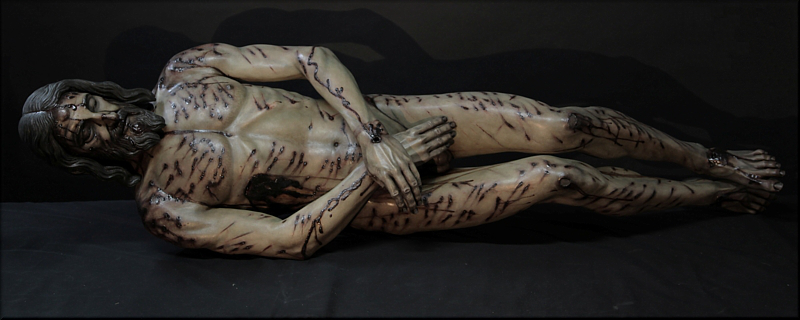
\includegraphics[width=1.0\textwidth]{minarro1.jpg}
    \caption{Cristo yacente de Miñarro: vista frontal.} %. URL: http://www.lahornacina.com/articulosminarro.htm
\end{figure}

\begin{figure}[ht!]
    \centering
    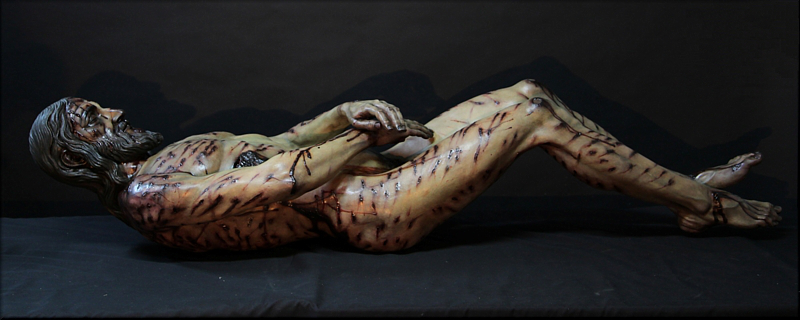
\includegraphics[width=1.0\textwidth]{minarro2.jpg}
    \caption{Cristo yacente de Miñarro: perfil.} %. URL: http://www.lahornacina.com/articulosminarro.htm
\end{figure}

\begin{figure}[ht!]
    \centering
    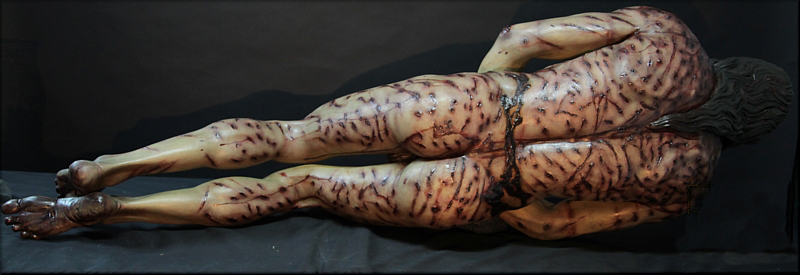
\includegraphics[width=1.0\textwidth]{minarro3.jpg}
    \caption{Cristo yacente de Miñarro: vista dorsal.} %. URL: http://www.lahornacina.com/articulosminarro.htm
\end{figure}

\newpage

\begin{description}
\item[Cronología:] 2012
\item[Lugar:] Exposición Sábana Santa (Itinerante)
\item[Estilo:] Realismo
%\item[Autor] Juan Manuel Miñarro
%\item[Título] Cristo de la Síndone o Sindónico
\end{description}

\textbf{Contexto histórico:} Esta obra es finalizada alrededor del año 2010, tras años empleados por el autor en su elaboración junto con otras esculturas que siguen la misma temática. Tanto es así, que existe otra figura de este mismo autor que reproduce el mismo Cristo pero en el momento de la crucifixión, en lugar de una vez fallecido (ver anexo\autoref{app:crucificadominarro}). El autor pretende mostrar lo más fielmente y científicamente posible la realidad de la muerte de Cristo. Se basa, por tanto, en una de las reliquias más conocidas, junto con el sudario de Oviedo, que posee relación con la muerte de Cristo: la Síndone de Turín o Sábana Santa (ver anexo\autoref{app:sindone}), realizando mediante el estudio meticuloso de ésta una impresionante escultura.

Aunque no está demostrado científicamente que la Síndone fuese la sábana que envolvió a Cristo tras su muerte, presenta ciertas características que han hecho que los expertos y estudiosos de todo el mundo la identifiquen como tal. Una característica que contribuye a ello es la propia imagen que conserva grabada, que por un lado posee las características propias de un hombre torturado y crucificado de la misma forma que Cristo según los evangelios, y que por otro lado se considera imposible de falsificar con las técnicas de las que se disponen hoy en día y más difícilmente aún en cualquier época anterior, puesto que es algo no se puede crear ni de forma natural ni de forma artificial.

En su búsqueda de la realidad el autor refleja de forma impecable las heridas, contusiones, laceraciones y demás aspectos que proveen a la obra de un dramatismo nunca visto hasta ahora en la muerte de Cristo ni en obras pictóricas ni escultóricas. Además plasma todos aquellos detalles que identifican a Cristo como un hombre torturado a la hora de su muerte.

\vspace{12pt}
\textbf{Anatomía de superficie:}

En esta obra se nos muestra a un Cristo muy estudiado desde absolutamente todas y cada una de las perspectivas desde las que se puede tener en cuenta: en su anatomía, en la reproducción de la muerte y en la representación de las heridas y contusiones.

Al centrarnos en el primer punto se puede observar una figura proporcionada, y anatómicamente coherente con el conocimiento anatómico actual y con la imagen de la Síndone, mediante la cual el autor ha logrado producir la silueta y los detalles de Cristo en su muerte de una forma realista. Se llega incluso a considerar la altura de Cristo sobre el metro ochenta, plasmando este aspecto también en la escultura.

Además, el autor refleja con gran detalle las lesiones de Cristo.

Podemos apreciar los hasta 120 latigazos de los que, supuestamente, fue víctima antes de ser crucificado y que están grabados con todo detalle en la piel de esta figura.

Los orificios provocados por los clavos pueden apreciarse en ambas muñecas, en la región carpiana, según la creencia actual, en lugar de en las palmas de las manos, entre los metacarpos. Y en los pies, que se cree que fueron clavados juntos con un solo clavo, debido a las características que presenta la Síndone, los orificios se encuentran en el punto de confluencia del calcáneo, astrágalo, escafoides y cuboides.

Igualmente se puede casi asegurar por la posición de los pies, el izquierdo flexionado unos noventa grados y el derecho extendido alrededor de ciento cincuenta y cinco grados, que el primero se encontraba sobre el segundo en el momento de la crucifixión.

En el rostro presenta un gran hematoma en el lado derecho, que se extiende desde debajo del arco cigomático hasta el ojo. Presenta también una rotura del tabique nasal. Ambas lesiones pudieron deberse a los puñetazos que le pegaron ante Caifás antes de ser condenado, o una bofetada según dice el evangelio de Juan (Jn 18, 22; Lc 22, 63; Mc 14, 65; Mt 26, 67), o incluso deberse a alguna caída en su recorrido al monte Calvario, ya que al llevar a cuestas el \textit{patibulum} no podría parar la caída con las extremidades superiores.

En la frente el autor nos muestra las heridas de la corona de espinas que continúan hacia la zona occipital de la cabeza, aunque son menos apreciables al estar cubiertas por el cabello.

No dejándose ningún detalle por el camino, el autor nos muestra las excoriaciones de las rodillas a la altura de la rótula, que podrían coincidir con las tres supuestas caídas de Cristo durante el camino al monte Calvario cargado con la cruz, que si bien no aparecen relatadas en la Biblia, sí que parecen obvias en la Síndone.

Así mismo el autor diferencia la proveniencia de la sangre, es decir, si Cristo todavía estaba vivo o si, por el contrario, ya estaba muerto cuando se produjo cada herida. Por ejemplo, en la herida del costado derecho producida por la lanza y situada por el autor entre la quinta y la sexta costilla, refleja el aspecto que podría tomar una herida postmortem, apreciándose la sangre como una masa coagulada y separada parcialmente del plasma, éste de un color más claro. La sangre proveniente de esta herida recorre, además, la zona lumbar de la espalda a modo de cinturón, como resultado del movimiento de Cristo de la cruz al sepulcro.

Claramente se trata de una figura que representa a Cristo muerto una vez producido el descendimiento de Cristo de la Cruz.

La figura mantiene una postura rígida provocada por el \textit{rigor mortis}, que se cree pudo empezar a originarse poco después de la muerte de Cristo, como ocurre en aquellas personas que han sido sometidas a grandes esfuerzos o actividad extenuante. De hecho es probable que el \textit{rigor mortis} comenzase cuando Cristo aún se encontraba suspendido en la cruz. Por ello podemos observar que las extremidades inferiores conservan la posición en la que estarían en ese momento.

Sin embargo la posición de los brazos no es la que tendría un crucificado que ha permanecido en la cruz durante el \textit{rigor mortis}: brazos casi completamente extendidos, en abducción y supinación del antebrazo, por lo que se asume que las extremidades superiores fueron forzadas antes de producirse el \textit{rigor mortis} completo, momento en el que la movilización de éstos habría sido imposible sin desgarrar tejidos. 

Otro detalle perteneciente a las extremidades superiores es que los primeros dedos de ambas manos se encuentran dispuestos sobre las palmas de las manos debido a una posible lesión del nervio mediano al introducir los clavos, aunque también podría ser la posición normal del primer dedo en la relajación muscular, que precede al \textit{rigor mortis}, por acción de los músculos flexores.

Debido a la contracción algunos músculos se aprecian más prominentes que en su estado habitual, es el caso de los músculos pectorales mayores, dando un aspecto de tórax distendido que contrasta con el vientre hundido de la figura, que hace posible la visión del borde costal inferior, así como parte de la caja torácica.

El crucificado muestra en las plantas de ambos pies un característico color azulado propio del \textit{livor mortis}. Éste consiste precisamente en la acumulación de la sangre por el efecto de la gravedad en las partes inferiores del cuerpo, según la posición de éste, proporcionando a la vez un color amarillento-ceniciento al resto del cuerpo por el que la sangre ya no fluye debido a la ausencia de latido cardíaco.

La figura estudiada demuestra que Cristo se mantuvo en la cruz después de muerto el tiempo suficiente como para que la sangre por efecto de la gravedad quedase retenida en la zona inferior de los miembros inferiores. Aunque no demasiado tiempo, pues en tal caso la cantidad de sangre acumulada en las extremidades inferiores sería superior, aun teniendo en cuenta la abundante sangre perdida antes y durante la crucifixión.

Además, queda patente que el cuerpo no ha permanecido en decúbito supino durante largo tiempo, ya que en tal caso la sangre también se habría acumulado en las zonas inferiores, en este caso la parte posterior de la figura.
\section{Resultados y discusión}
\section{Conclusión}
Tras haber realizado el análisis de varias obras de distintas épocas se pueden sacar varias ideas en claro.

Las obras se rigen por el estilo predominante de la época, aunque en ocasiones los autores de éstas aporten novedades en el arte de su tiempo, como Mantegna que revolucionó la perspectiva con su lamentación sobre Cristo muerto o Dalí con su estilo único.

La intención del autor también cambia. Algunos autores intentan mostrar una obra bella utilizando para ello proporciones y armonía, como Velázquez o Dalí, mientras que otros utilizan la prevalencia del realismo para crear una obra que represente la muerte de Cristo de una forma lo más exacta posible a la realidad, éste es el caso de Mantegna o Miñarro.

En relación a la anatomía, %se ve diferencia entre aquellas obras anteriores a las disecciones del cuerpo y aquellas en las que el conocimiento del cuerpo era mayor.
la figura de la obra de Mantegna posee una anatomía estudiada, sin embargo no es en lo que más se centra, numerosos detalles en la obra son más impresionantes, como la perspectiva que adopta la figura de Cristo o los rasgos referentes a la muerte que éste presenta. Velázquez sí que se centra mucho en la anatomía superficial y en las proporciones del Cristo de su obra. Dalí, por su parte, se propone dibujar el Cristo más bello, para el que adopta una perspectiva nueva e incluso se dice que utiliza un modelo para representar de forma correcta la anatomía. Miñarro, por su parte, se basa en la Síndone de Turín para intentar representar la muerte de Cristo como nunca hasta ahora se había visto, en toda su crudeza.

%El número de clavos con el que Cristo aparece clavado en la Cruz es variable debido, más a las ideas del propio autor que a las de la época. De hecho, en todas las obras analizadas se puede observar la inserción de tres clavos, uno uniendo los dos pies y otro en cada extremidad superior, excepto en la obra de Velázquez que se deja influir por su maestro, y no así por su tiempo. Otro detalle sobre la inserción de los clavos es que a lo largo del tiempo el Evangelio de San Juan ha sido interpretado de forma que incluso en épocas más modernas estos se han seguido representado en la palma de la mano y no ha sido hasta hace varias décadas que se han hecho experimentos en cuanto a ello. Por ello, en la obra de Miñarro es en la única que se pueden apreciar los clavos a la altura de los carpos y no entre los metacarpos como se representa en las demás obras.

En cuanto a la representación de la muerte de Cristo, Mantegna en su obra presenta la laxitud en la postura y la rigidez en algunos músculos, que probablemente está relacionada con el \textit{rigor mortis}, además de la lividez con la que el autor ilustra el cuerpo, reproduciendo de manera bastante acertada la apariencia de un cadáver.

Velázquez, sin embargo, realiza una obra en la que no reproduce la muerte de Cristo. El Cristo no posee ninguna característica de un cuerpo muerto, ni laxitud en los músculos ni lividez cadavérica. Es más, muestra ciertas características que nos llevan a la conclusión de que el Cristo no ha fallecido e icluso se encuentra en relativas buenas condiciones, sobre todo, tratándose de una figura que ha soportado toda clase de martirios.

Dalí propone la imagen de un Cristo que no porta nungún elemento utilizado para su suplicio ni crucifixión. Aún así, nos muestra una cristo cuyos músculos están relajados, como si estuviese a punto de fallecer o ya hubiera fallecido. En cuanto a la coloración del cuerpo, es dificil de determinar si posee el característico del \textit{livor mortis} o no, debido al gran contraste de luz que Dalí utiliza en la obra.

En el Cristo de la Síndone de Miñarro se distinguen fácilmente las características de la muerte en la figura. De hecho ésta posee un \textit{rigor mortis} con una rigidez muy marcada y un \textit{livor mortis} que se aprecia en el color ceniciento del cuerpo, así como en el acúmulo de sangre en la zona más distal de las extremidades inferiores.

\nocite{*} % Show all Bib-entries
\bibliographystyle{vancouver}
\bibliography{bibliography}

\clearpage
\begin{appendices}
\let\clearpage\relax
\section{Hombre de Vitruvio} \label{app:vitruvio}

\begin{figure}[H]
    \centering
    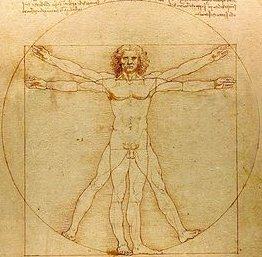
\includegraphics[width=0.35\textwidth]{vitruvio2.jpg}
    \caption{Hombre de Vitruvio, el dibujo más conocido de Leonardo Da Vinci.\cite{RefWorks:71}} % URL:http://upload.wikimedia.org/wikipedia/commons/thumb/2/22/Da_Vinci_Vitruve_Luc_Viatour.jpg/300px-Da_Vinci_Vitruve_Luc_Viatour.jpg  http://commons.wikimedia.org/wiki/File:Da_Vinci_Vitruve_Luc_Viatour.jpg#mediaviewer/Archivo:Da_Vinci_Vitruve_Luc_Viatour.jpg
\end{figure}

\section{Andrés Vesalio} \label{app:vesalio}

Andrés Vesalio fue un pionero en el ámbito de la anatomía. En su tratado ``De humani corporis fabrica'' se pueden apreciar diversas representaciones de la anatomía del cuerpo humano en movimiento. A continuación están detallados algunos de estos dibujos:
\begin{figure}[H]
    \centering
        \begin{subfigure}[b]{0.28\textwidth}
             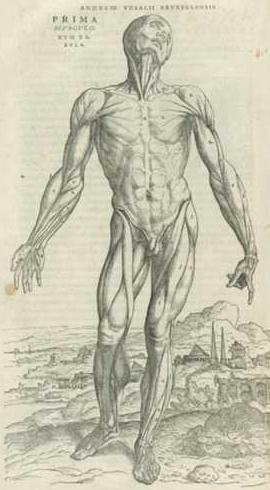
\includegraphics[height=6cm]{musculos.jpg}
             \caption{Músculos\cite{RefWorks:41}}
        \end{subfigure}
        \begin{subfigure}[b]{0.28\textwidth}
             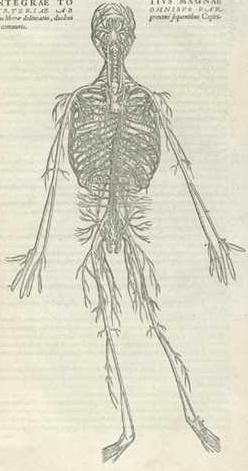
\includegraphics[height=6cm]{nervios.jpg}
             \caption{Nervios\cite{RefWorks:41}}
        \end{subfigure}
        \begin{subfigure}[b]{0.28\textwidth}
            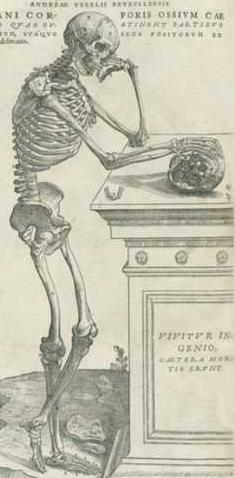
\includegraphics[height=6cm]{esqueleto.jpg}
            \caption{Esqueleto\cite{RefWorks:41}}
        \end{subfigure}
        \begin{subfigure}[b]{0.37\textwidth}
             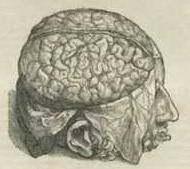
\includegraphics[width=\textwidth]{cabeza.jpg}
             \caption{Cabeza y cerebro\cite{RefWorks:41}}
        \end{subfigure}
        \begin{subfigure}[b]{0.3\textwidth}
             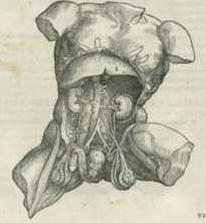
\includegraphics[width=\textwidth]{interior.jpg}
             \caption{Órganos internos\cite{RefWorks:41}}
        \end{subfigure}
\end{figure}
% http://www.biografiasyvidas.com/biografia/v/vesalio.htm
% http://archive.nlm.nih.gov/proj/ttp/flash/vesalius/vesalius.html
% http://quod.lib.umich.edu/w/wantz/vesd1.htm
% Andrés Vesalio, su vida y su obra Escrito por José Barón Fernández

\section{Tipos de Cruces} \label{app:crosses}

Tradicionalmente existen cuatro tipos de cruces según su morfología específica básica. Estos cuatro modelos son:
%\begin{itemize}
%\item[La cruz Latina, cruz immissa o cruz ordinaria]
%\item[La cruz Griega o cruz immissa quadrata]
%\item[La cruz de San Andrés o cruz decussata]
%\item[La cruz Tau, cruz commissa o en forma de T]
%\end{itemize}

\begin{description}
\item[] La cruz Latina, cruz \textit{Immissa} o cruz ordinaria
\item[] La cruz Griega o cruz \textit{Immissa quadrata}
\item[] La cruz de San Andrés o cruz \textit{Decussata}
\item[] La cruz Tau, cruz \textit{Commissa} o en forma de T
\end{description}


\begin{figure}[H]
    \centering
    
\includegraphics[width=1\textwidth]{cruces.jpg}
    \caption{Distintos tipos de cruces.\cite{RefWorks:43}} % URL:http://www.crosses.org/history.htm
\end{figure}

\section{Cristo de San Juan de la Cruz} \label{app:sanjuan}

\begin{figure}[H]
    \centering
    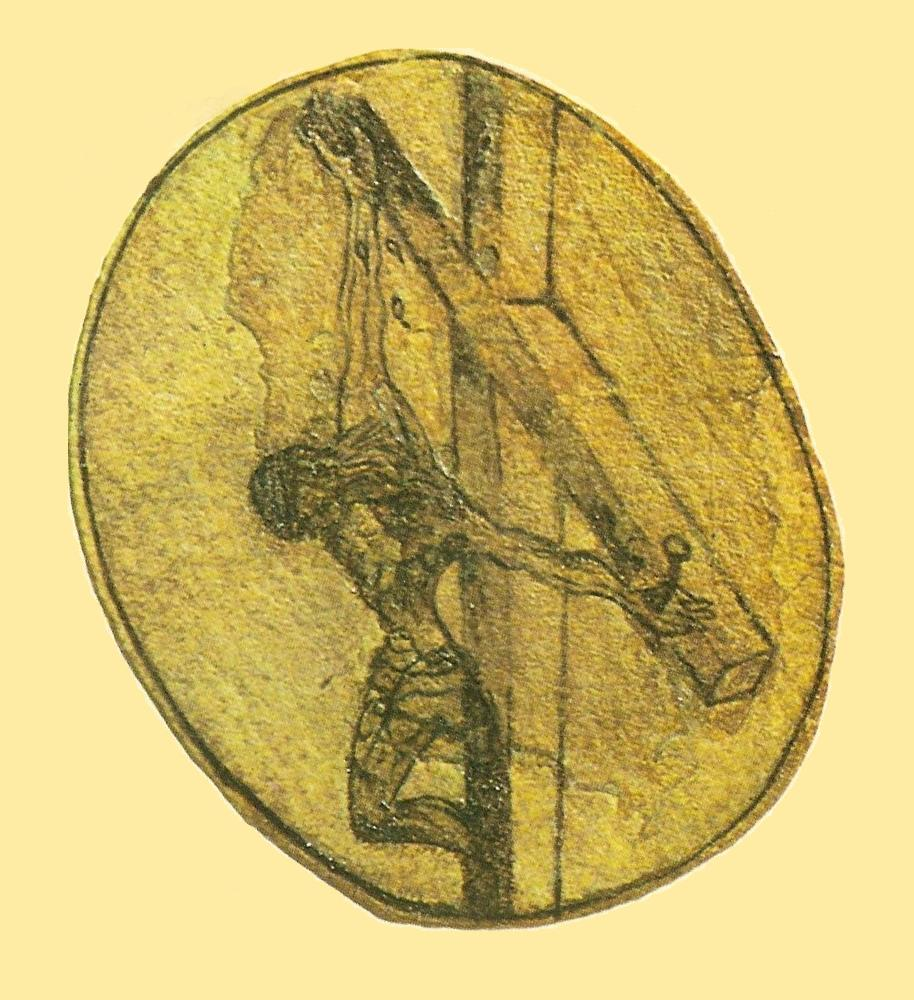
\includegraphics[width=0.55\textwidth]{sanju.jpg}
    \caption{Cristo original de San Juan de la Cruz, que inspiró a Dalí en su obra.\cite{RefWorks:44}} % URL:http://archipielagoduda.blogspot.com.es/2011/03/el-unico-dibujo-conservado-de-san-juan.html
\end{figure}

\section{Cristo Crucificado de la Hermandad Universitaria de Córdoba} \label{app:crucificadominarro}

Este Cristo crucificado realizado por Juan Manuel Miñarro se encuentra en la Hermandad Universitaria de Córdoba y sirve de paso de semana santa en las procesiones de esta ciudad.

\begin{figure}[H]
    \centering
    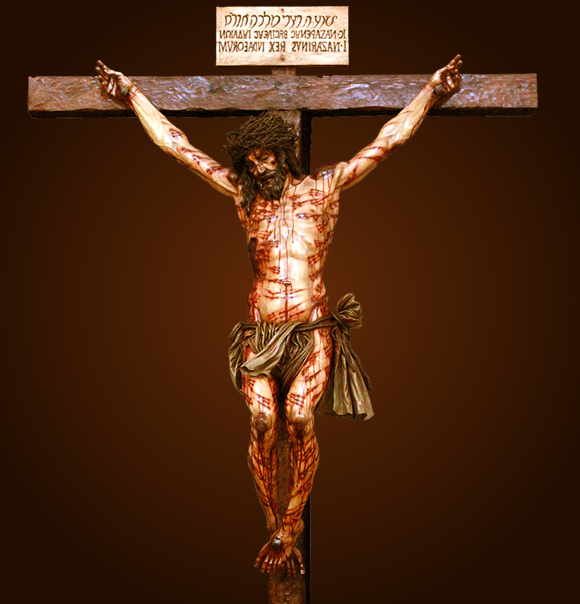
\includegraphics[width=0.6\textwidth]{crucificadominarro.jpg}
    \caption{Escultura de Cristo crucificado realizada por Miñarro.\cite{RefWorks:70}} % URL: http://hermandaduniversitaria.files.wordpress.com/2012/04/sesion5_big.jpg
\end{figure}

\section{La Síndone de Turín o Sábana Santa} \label{app:sindone}

\begin{figure}[H]
    \centering
    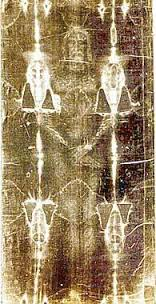
\includegraphics[width=0.29\textwidth]{sindone.jpg}
    \caption{Tela de lino que posee grabada la imagen de un hombre con marcas de martirio y crucifixión. Se cree que pudo envolver a Cristo tras su muerte.\cite{RefWorks:72}} % URL:http://www.lanuovaregaldi.it/photo/eventi/sindonetorino.jpg
\end{figure}


\end{appendices}

\end{document}
